\newpage

\begin{center}
\textsc{Figure \ref{fig:workflow}}
\end{center}
Stylized DateLife workflow. This shows the general worflows and analyses that can be performed with \texttt{datelife}, via the R package or through the website. Details on the functions involved on each workflow are shown in \texttt{datelife}'s R package vignette.

\begin{center}
\textsc{Figure \ref{fig:runtime1}}
\end{center}
Computation time of query processing and search across \texttt{datelife}'s chronogram database relative to number of input taxon names. We sampled N names from the class Aves for each cohort 100 times and then performed a search with query processing not using the Taxon Names Resoultion Service (TNRS; dark gray), and using TNRS (light gray). We also performed a search using the already processed query for comparison (light blue). 

\begin{center}
\textsc{Figure \ref{fig:schronograms1}}
\end{center}
Lineage through time (LTT) plots of source chronograms containing all or a subset of species from the bird family Fringillidae of true finches. Arrows indicate maximum age of each chronogram. Numbers reference to chronograms' original publications 1: Barker et al. (\protect\hyperlink{ref-barker2012going}{2012}), 2: Barker et al. (\protect\hyperlink{ref-barker2015new}{2015}), 3: Burns et al. (\protect\hyperlink{ref-burns2014phylogenetics}{2014}), 4: Claramunt and Cracraft (\protect\hyperlink{ref-claramunt2015new}{2015}), 5: Gibb et al. (\protect\hyperlink{ref-gibb2015new}{2015}), 6: Hedges et al. (\protect\hyperlink{ref-Hedges2015}{2015}), 7: Hooper and Price (\protect\hyperlink{ref-hooper2017chromosomal}{2017}), 8: Jetz et al. (\protect\hyperlink{ref-Jetz2012}{2012}), 9: Price et al. (\protect\hyperlink{ref-price2014niche}{2014}).

\begin{center}
\textsc{Figure \ref{fig:summaries}}
\end{center}
LTT plots of median and Supermatrix Distance Method (SDM) chronograms summarising information from source chronograms found for the Fringillidae. Arrows indicate maximum age.

\begin{center}
\textsc{Figure \ref{fig:cvbladj}}
\end{center}
LTT plots showing results from the cross-validation analyses of trees without branch lengths dated using BLADJ. The dating analysis can only be performed in trees with more than 2 tips, thus excluding chronogram from study 4; its data was still used as calibration for the other source chronograms.

\begin{center}
\textsc{Figure \ref{fig:cvbold}}
\end{center}
LTT plots showing results from the cross-validation analyses of trees with branch length reconstructed with data from the Barcode of Life Database (BOLD) dated using PATHd8. We could construct a tree with branch lengths for all source chronograms. However, dating with PATHd8 was only successful in three source chronograms shown here.

\newpage

\begin{figure}[!h]
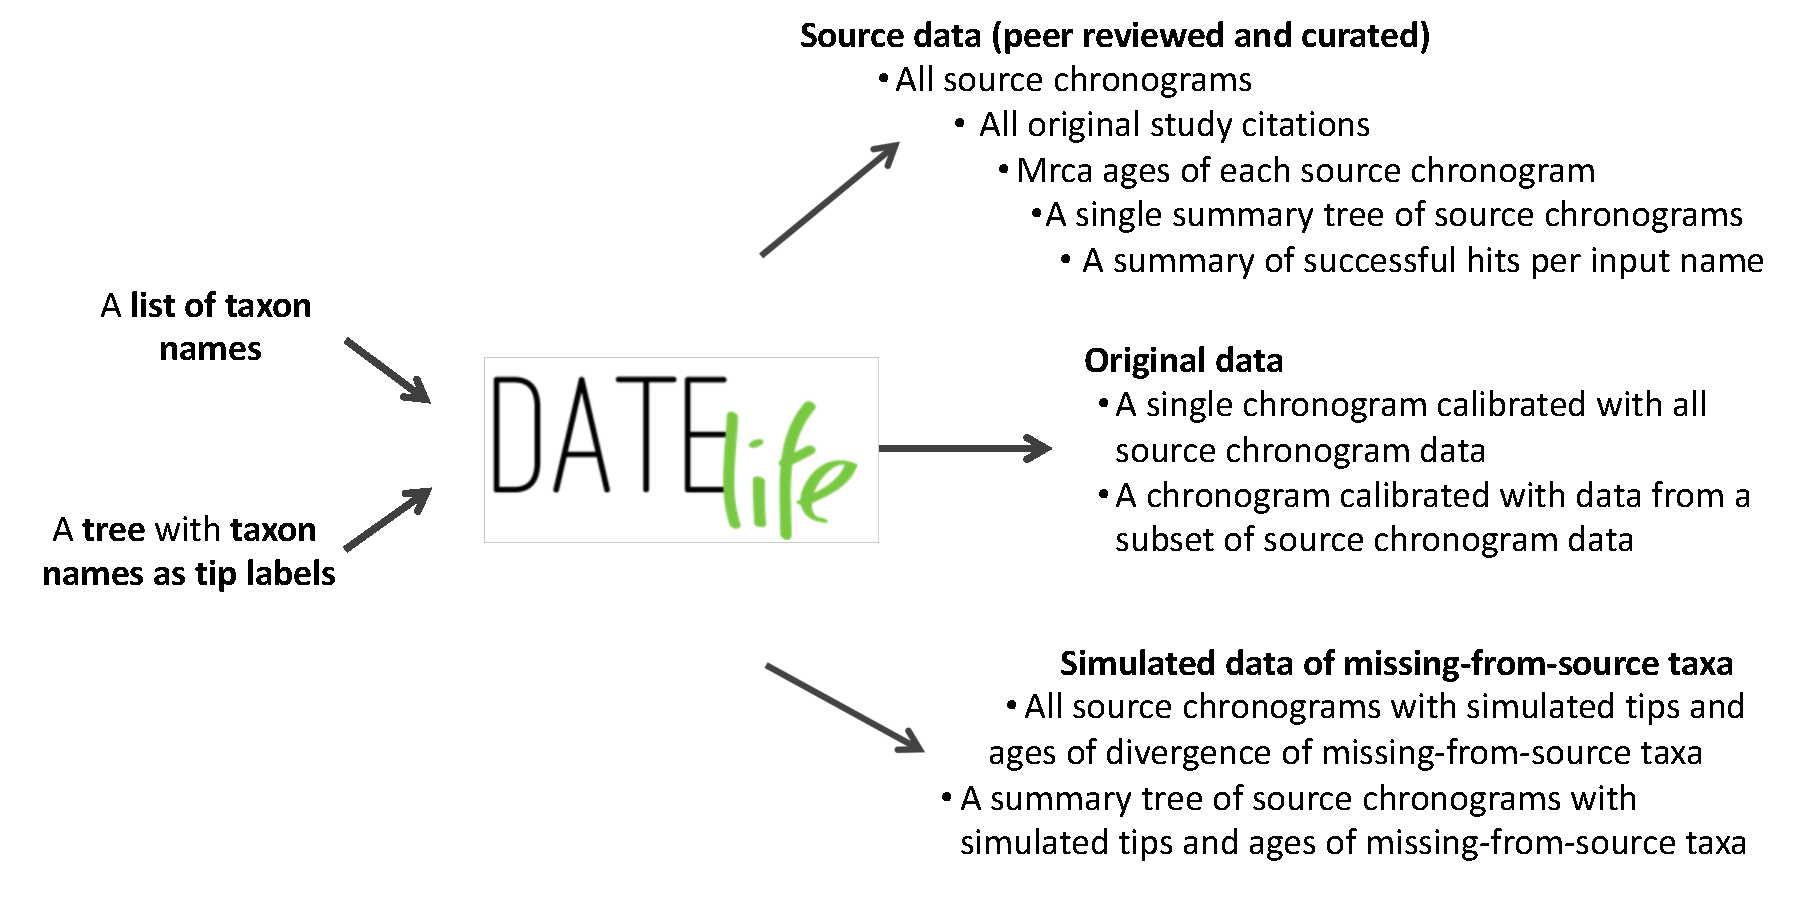
\includegraphics{Fig1.pdf}
\caption{}
\label{fig:workflow}
\end{figure}

\newpage

\begin{figure}[!h]
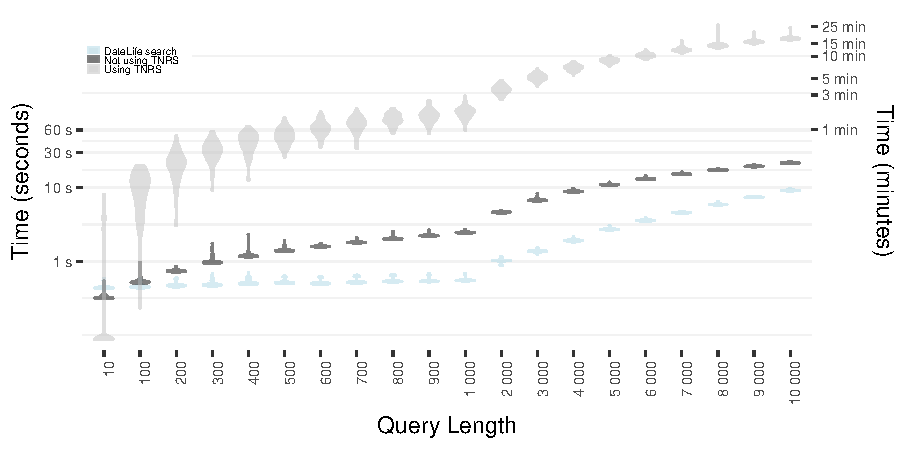
\includegraphics[width=1\linewidth]{fig_runtime_main.pdf}
\caption{}
\label{fig:runtime1}
\end{figure}

\newpage

\begin{figure}[!h]
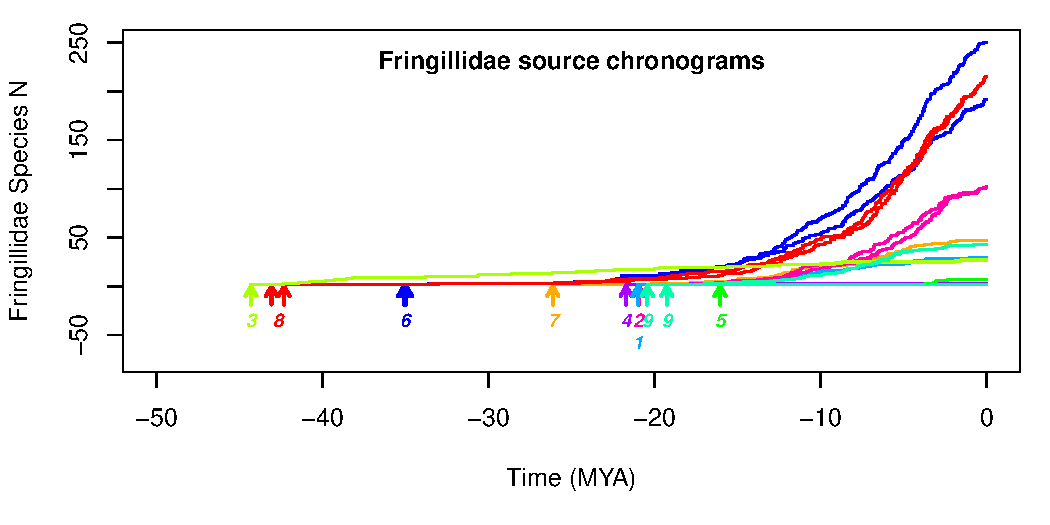
\includegraphics[width=1\linewidth]{fig_schronograms1.pdf}
\caption{}
\label{fig:schronograms1}
\end{figure}

\newpage

\begin{figure}[!h]
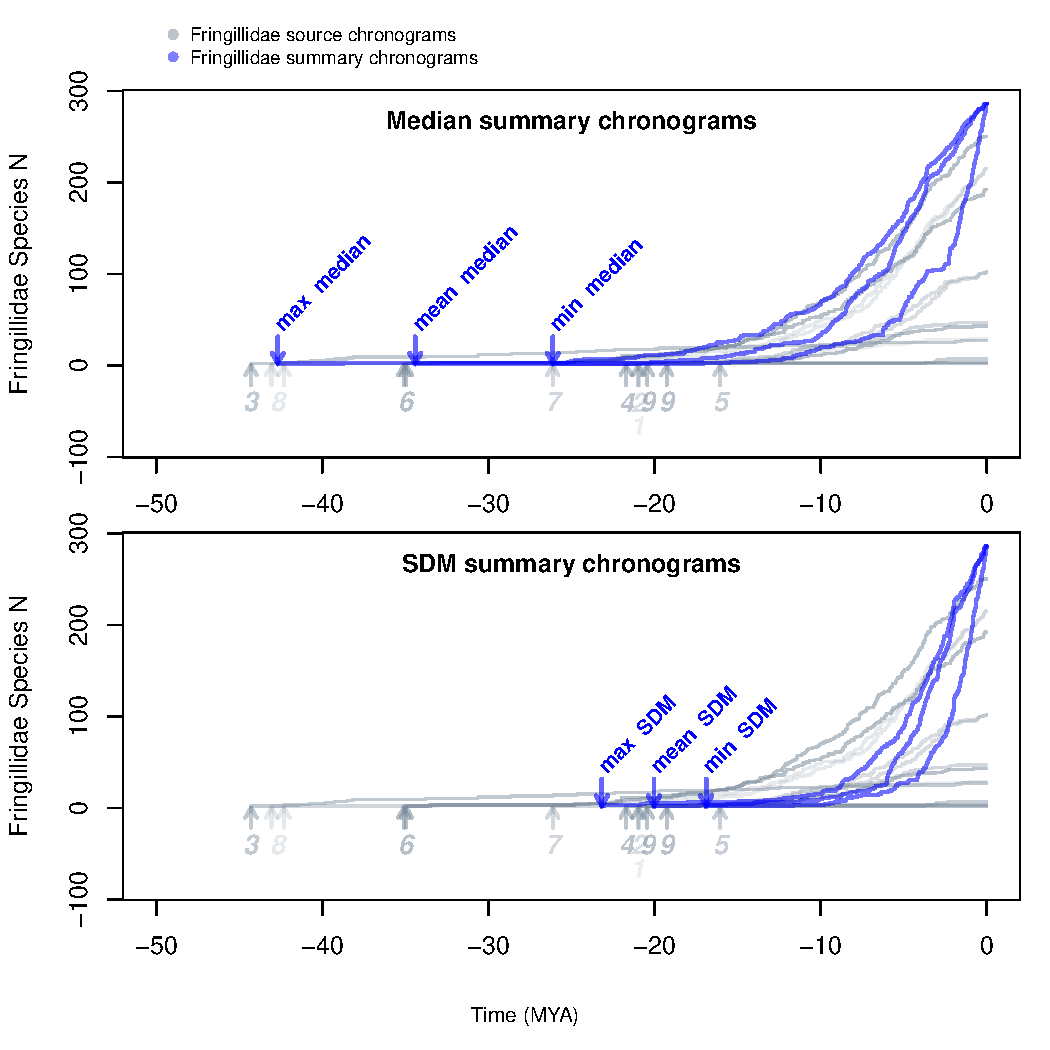
\includegraphics{fig_summaries.pdf}
%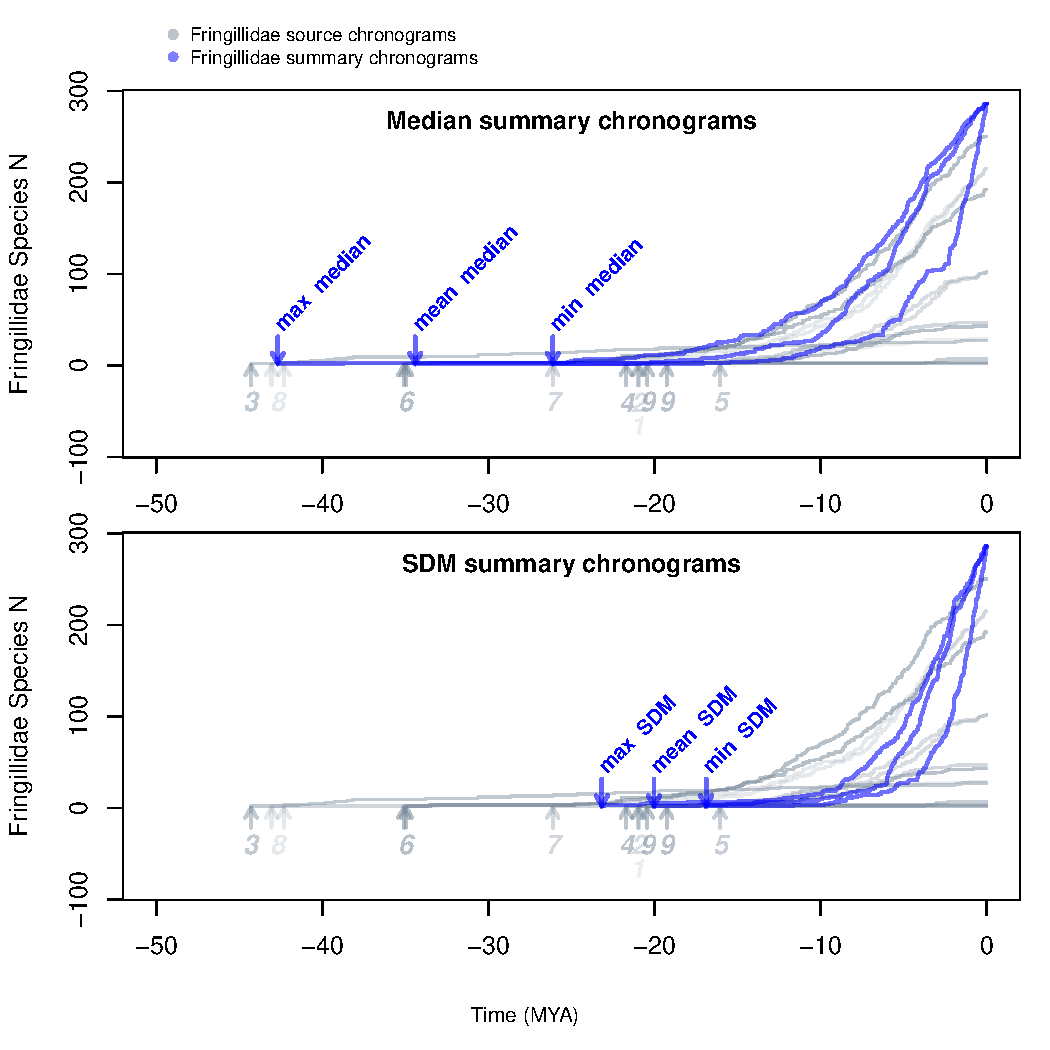
\includegraphics{fig_summaries.pdf}
\caption{}
\label{fig:summaries}
\end{figure}

\newpage

\begin{figure}[!h]
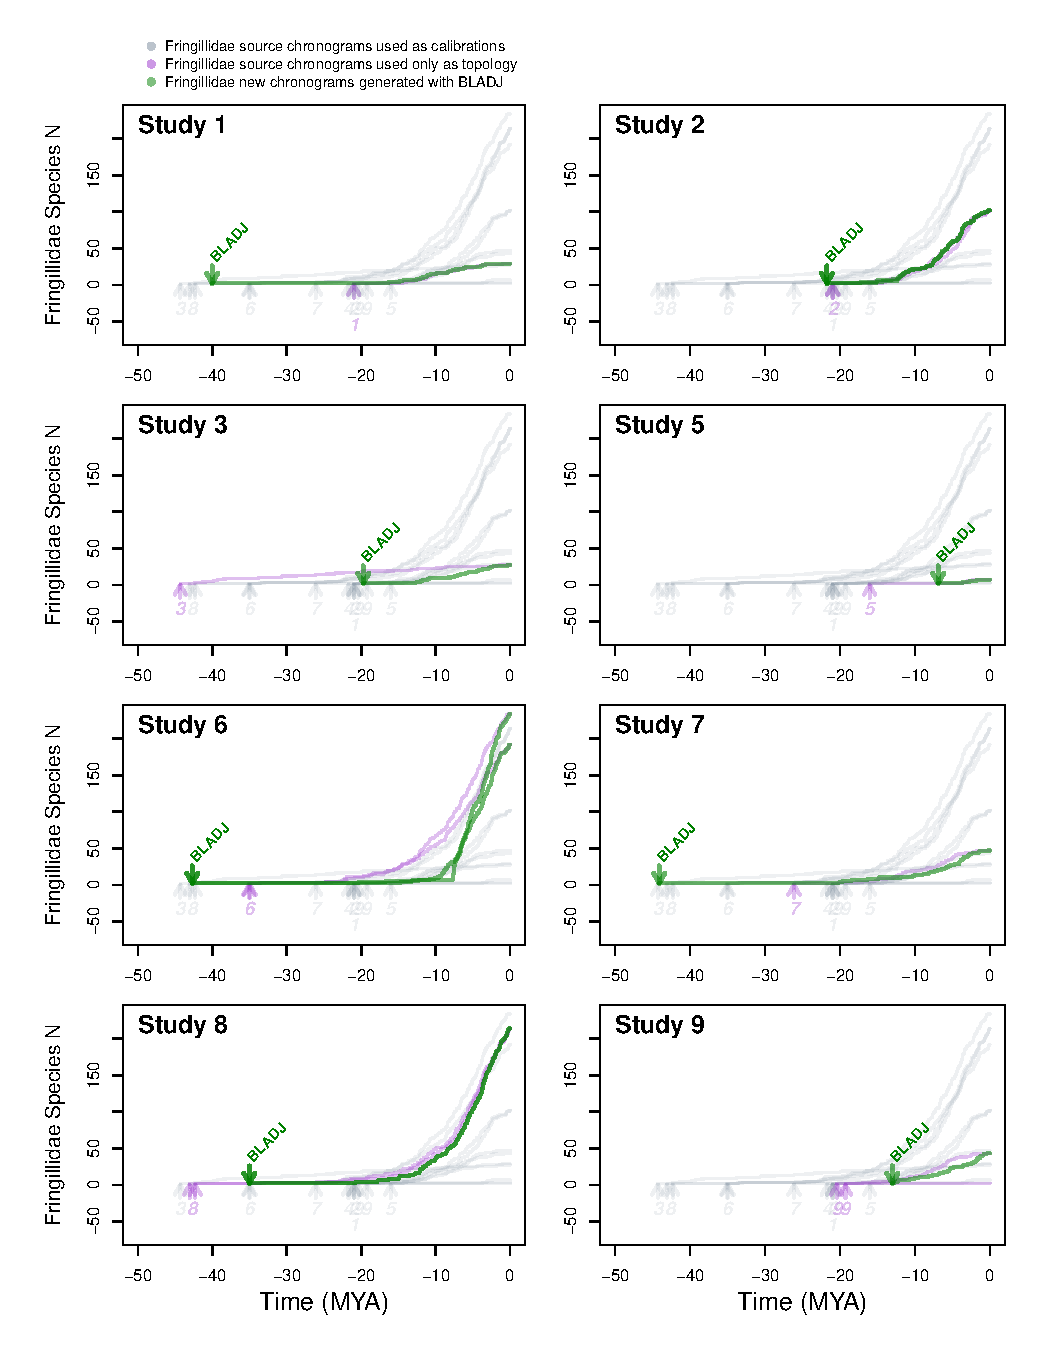
\includegraphics{fig_crossval_bladj.pdf}
\caption{}
\label{fig:cvbladj}
\end{figure}

\newpage

\begin{figure}[!h]
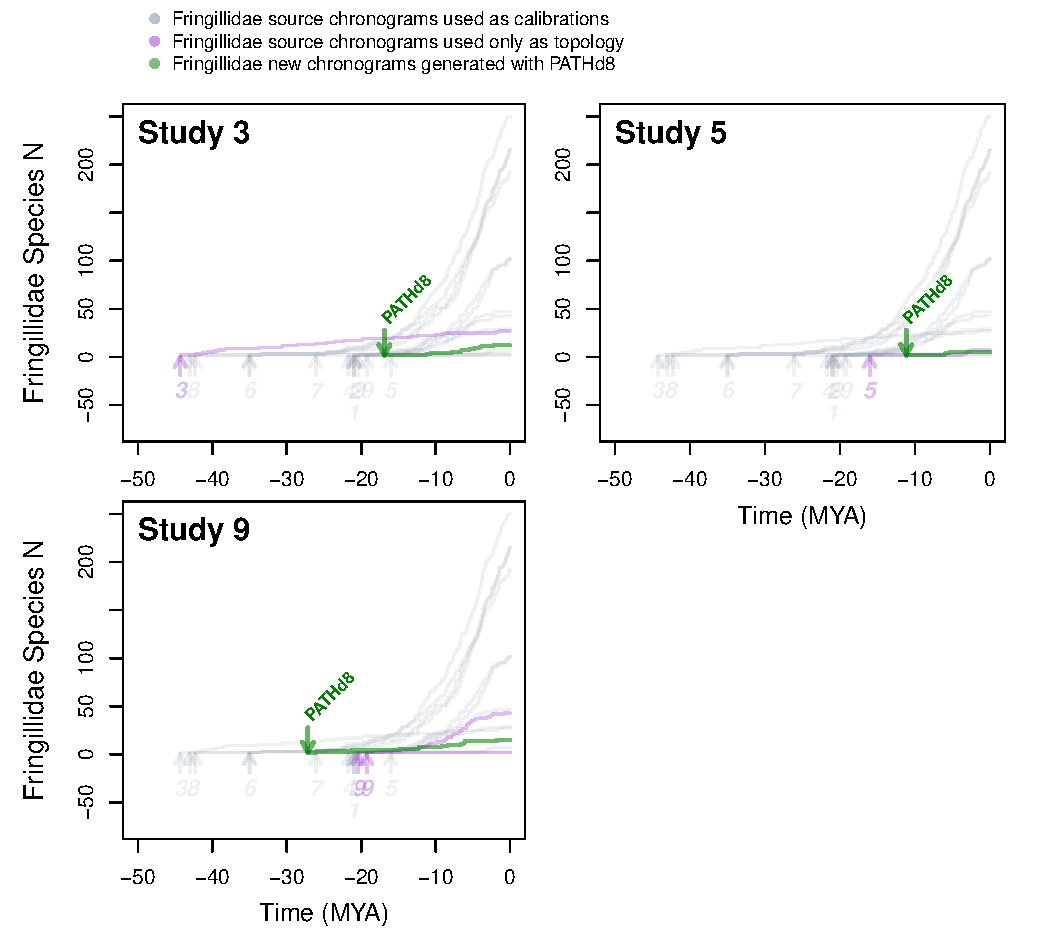
\includegraphics{fig_crossval_boldsumm.pdf}
\caption{}
\label{fig:cvbold}
\end{figure}




